\documentclass[a4paper, 12pt]{article}
% packages
\usepackage{amssymb}
\usepackage[fleqn]{mathtools}
\usepackage{tikz}
\usepackage{enumerate}
\usepackage{bussproofs}
\usepackage{xcolor}
\usepackage[margin=1.3cm]{geometry}
\usepackage{logicproof}
\usepackage{diagbox}
\usepackage{listings}
\usepackage{graphicx}
\usepackage{lstautogobble}
\usepackage{hyperref}
\usepackage{multirow}
\usetikzlibrary{arrows, shapes.gates.logic.US, circuits.logic.US, calc, automata, positioning}

% shorthand for verbatim
% this clashes with logicproof, so maybe fix this at some point?
\catcode`~=\active
\def~#1~{\texttt{#1}}

% code listing
\lstdefinestyle{main}{
    numberstyle=\tiny,
    breaklines=true,
    showspaces=false,
    showstringspaces=false,
    tabsize=2,
    numbers=left,
    basicstyle=\ttfamily,
    columns=fixed,
    fontadjust=true,
    basewidth=0.5em,
    autogobble,
    xleftmargin=3.0ex,
    mathescape=true
}
\newcommand{\dollar}{\mbox{\textdollar}} %
\lstset{style=main}

% augmented matrix
\makeatletter
\renewcommand*\env@matrix[1][*\c@MaxMatrixCols c]{%
\hskip -\arraycolsep
\let\@ifnextchar\new@ifnextchar
\array{#1}}
\makeatother

% ceiling / floor
\DeclarePairedDelimiter{\ceil}{\lceil}{\rceil}
\DeclarePairedDelimiter{\floor}{\lfloor}{\rfloor}

% custom commands
\newcommand{\indefint}[2]{\int #1 \, \mathrm{d}#2}
\newcommand{\defint}[4]{\int_{#1}^{#2} #3 \, \mathrm{d}#4}
\newcommand{\dif}[2]{\frac{\mathrm{d}#1}{\mathrm{d}#2}}
\newcommand{\limit}[2]{\raisebox{0.5ex}{\scalebox{0.8}{$\displaystyle{\lim_{#1 \to #2}}$}}}
\newcommand{\summation}[3]{\sum\limits_{#1}^{#2} #3}
\newcommand{\intbracket}[3]{\left[#3\right]_{#1}^{#2}}
\newcommand{\ulsmash}[1]{\underline{\smash{#1}}}

\newcommand{\powerset}[0]{\wp}
\renewcommand{\emptyset}[0]{\varnothing}

\makeatletter
\newsavebox{\@brx}
\newcommand{\llangle}[1][]{\savebox{\@brx}{\(\m@th{#1\langle}\)}%
  \mathopen{\copy\@brx\kern-0.5\wd\@brx\usebox{\@brx}}}
\newcommand{\rrangle}[1][]{\savebox{\@brx}{\(\m@th{#1\rangle}\)}%
  \mathclose{\copy\@brx\kern-0.5\wd\@brx\usebox{\@brx}}}
\makeatother
\newcommand{\lla}{\llangle}
\newcommand{\rra}{\rrangle}
\newcommand{\la}{\langle}
\newcommand{\ra}{\rangle}

\newcommand{\mat}[1]{\mathbf{#1}}
\newcommand{\rowt}[1]{\begin{bmatrix}
    #1
\end{bmatrix}^\top}

\newcommand{\unaryproof}[2]{\AxiomC{#1} \UnaryInfC{#2} \DisplayProof}
\newcommand{\binaryproof}[3]{\AxiomC{#1} \AxiomC{#2} \BinaryInfC{#3} \DisplayProof}
\newcommand{\trinaryproof}[4]{\AxiomC{#1} \AxiomC{#2} \AxiomC{#3} \TrinaryInfC{#4} \DisplayProof}

\newcommand{\axiom}[1]{\AxiomC{#1}}
\newcommand{\unary}[1]{\UnaryInfC{#1}}
\newcommand{\binary}[1]{\BinaryInfC{#1}}
\newcommand{\trinary}[1]{\TrinaryInfC{#1}}
\newcommand{\dproof}[0]{\DisplayProof}

\newcommand{\bnfsep}[0]{\ |\ }
\newcommand{\concsep}[0]{\ ||\ }
\newcommand{\violet}[1]{\textcolor{violet}{#1}}
\newcommand{\blue}[1]{\textcolor{blue}{#1}}
\newcommand{\red}[1]{\textcolor{red}{#1}}

% no indent
\setlength\parindent{0pt}

% reasoning proofs
\usepackage{ltablex}
\usepackage{environ}
\keepXColumns
\NewEnviron{reasoning}{
    \begin{tabularx}{\textwidth}{rlX}
        \BODY
    \end{tabularx}
}
\newcommand{\proofline}[3]{$(#1)$ & $#2$ & \hfill #3 \smallskip \\}
\newcommand{\proofarbitrary}[1]{& take arbitrary $#1$ \smallskip \\}
\newcommand{\prooftext}[1]{\multicolumn{3}{l}{#1} \smallskip \\}
\newcommand{\proofmath}[3]{$#1$ & = $#2$ & \hfill #3 \smallskip \\}
\newcommand{\prooftherefore}[1]{& $\therefore #1$ \smallskip \\}
\newcommand{\proofbc}[0]{\prooftext{\textbf{Base Case}}}
\newcommand{\proofis}[0]{\prooftext{\textbf{Inductive Step}}}

% reasoning er diagrams
\newcommand{\nattribute}[4]{
    \node[draw, state, inner sep=0cm, minimum size=0.2cm, label=#3:{#4}] (#1) at (#2) {};
}
\newcommand{\mattribute}[4]{
    \node[draw, state, accepting, inner sep=0cm, minimum size=0.2cm, label=#3:{#4}] (#1) at (#2) {};
}
\newcommand{\dattribute}[4]{
    \node[draw, state, dashed, inner sep=0cm, minimum size=0.2cm, label=#3:{#4}] (#1) at (#2) {};
}
\newcommand{\entity}[3]{
    \node[] (#1-c) at (#2) {#3};
    \node[inner sep=0cm] (#1-l) at ($(#1-c) + (-1, 0)$) {};
    \node[inner sep=0cm] (#1-r) at ($(#1-c) + (1, 0)$) {};
    \node[inner sep=0cm] (#1-u) at ($(#1-c) + (0, 0.5)$) {};
    \node[inner sep=0cm] (#1-d) at ($(#1-c) + (0, -0.5)$) {};
    \draw
    ($(#1-c) + (-1, 0.5)$) -- ($(#1-c) + (1, 0.5)$) -- ($(#1-c) + (1, -0.5)$) -- ($(#1-c) + (-1, -0.5)$) -- cycle;
}
\newcommand{\relationship}[3]{
    \node[] (#1-c) at (#2) {#3};
    \node[inner sep=0cm] (#1-l) at ($(#1-c) + (-1, 0)$) {};
    \node[inner sep=0cm] (#1-r) at ($(#1-c) + (1, 0)$) {};
    \node[inner sep=0cm] (#1-u) at ($(#1-c) + (0, 1)$) {};
    \node[inner sep=0cm] (#1-d) at ($(#1-c) + (0, -1)$) {};
    \draw
    ($(#1-c) + (-1, 0)$) -- ($(#1-c) + (0, 1)$) -- ($(#1-c) + (1, 0)$) -- ($(#1-c) + (0, -1)$) -- cycle;
}

% actual document
\begin{document}
    \section*{CO221 - Compilers}
        \subsection*{6th January 2020 \hfill Lecture}
            A compiler is a program which processes programs, including translating a program written in one language (usually higher level) to another programming language (usually in a lower level).
            In our course, the focus is to generate assembly code from the high level language.
            This translation goes between high level human concepts, and the data manipulation the machine performs.
            \subsubsection*{Structure}
                The general structure of a compiler is as follows;
                \begin{enumerate}[1.]
                    \itemsep0em
                    \item \textbf{input} \hfill takes in an input program in some language
                    \item \textbf{analysis} \hfill constructs an interal representation of the source structure
                    \item \textbf{synthesis} \hfill walks the representation to generate the output code
                    \item \textbf{output} \hfill creates an output in the target language
                \end{enumerate}
                In more detail, it can be represented as follows;
                \begin{center}
                    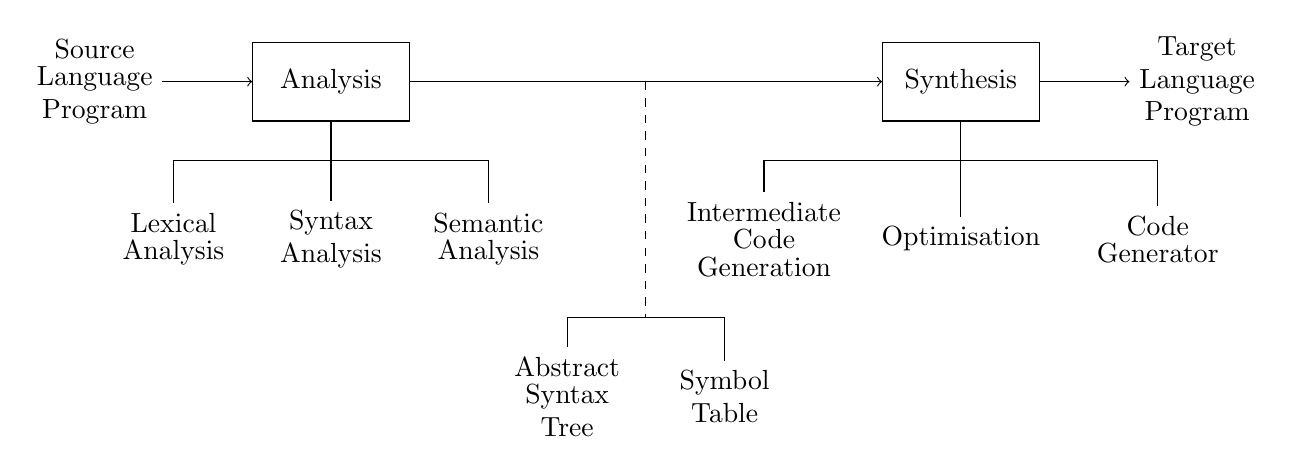
\begin{tikzpicture}
                        \node (slp) at (0, 0) {\shortstack{Source \\ Language \\ Program}};
                        \node (a) at (3, 0) {Analysis};
                        \node (s) at (11, 0) {Synthesis};
                        \node (tlp) at (14, 0) {\shortstack{Target \\ Language \\ Program}};

                        \node (la) at (1, -2) {\shortstack{Lexical \\ Analysis}};
                        \node (sa1) at (3, -2) {\shortstack{Syntax \\ Analysis}};
                        \node (sa2) at (5, -2) {\shortstack{Semantic \\ Analysis}};

                        \node (icg) at (8.5, -2) {\shortstack{Intermediate \\ Code \\ Generation}};
                        \node (o) at (11, -2) {Optimisation};
                        \node (cg) at (13.5, -2) {\shortstack{Code \\ Generator}};

                        \node (ast) at (6, -4) {\shortstack{Abstract \\ Syntax \\ Tree}};
                        \node (st) at (8, -4) {\shortstack{Symbol \\ Table}};

                        \draw
                        (slp) edge[->] (2, 0)
                        (4, 0) edge[->] (10, 0)
                        (12, 0) edge[->] (tlp)

                        (3, -0.5) -- (3, -1)
                        (11, -0.5) -- (11, -1)
                        (7, 0) edge[dashed] (7, -3)

                        (1, -1) -- (5, -1)
                        (1, -1) -- (la)
                        (3, -1) -- (sa1)
                        (5, -1) -- (sa2)

                        (8.5, -1) -- (13.5, -1)
                        (8.5, -1) -- (icg)
                        (11, -1) -- (o)
                        (13.5, -1) -- (cg)

                        (6, -3) -- (8, -3)
                        (6, -3) -- (ast)
                        (8, -3) -- (st)

                        (2, 0.5) -- (4, 0.5) -- (4, -0.5) -- (2, -0.5) -- cycle
                        (10, 0.5) -- (12, 0.5) -- (12, -0.5) -- (10, -0.5) -- cycle;
                    \end{tikzpicture}
                \end{center}
                \begin{itemize}
                    \itemsep0em
                    \item \textbf{lexical analysis} looks at characters of input program, analyses which are keywords (such as converting ~if~, and ~while~ to corresponding tokens), which are user defined words, and which are punctuation, etc.
                    \item \textbf{syntax analysis} discovers structure of input
                    \item \textbf{semantic analysis} checks that variables are declared before they are used, and that they are used consistently with their types etc.
                \end{itemize}
                Simple compilers go straight to code generation, but optimising compilers do several passes of intermediate code generation and optimisation.
                \smallskip

                The symbol table holds data on variables, such as types.
                Sometimes we need to know the type of the variable, in order to generate code for the variable, for example if we were to print a variable, it would need to generate different code for strings than it would need to do for integers.
                Scope rules are also needed.
            \subsubsection*{Phases}
                Whether all of these phases are done in the order shown is a design choice.
                For example, lexical analysis and syntax analysis are often interleaved.
                This can be done when the syntax analysis stage needs the next symbol, and therefore the lexical analysis stage can be used.
                \begin{center}
                    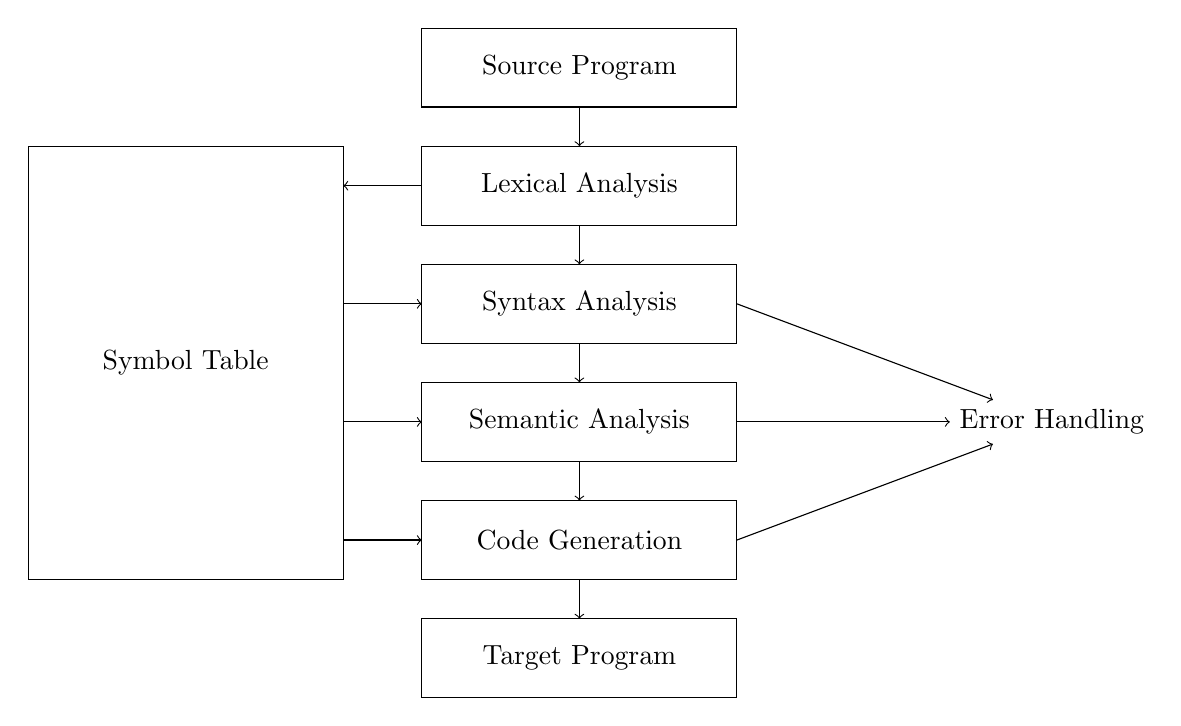
\begin{tikzpicture}
                        \node () at (0, 0) {Source Program};
                        \node () at (0, -1.5) {Lexical Analysis};
                        \node () at (0, -3) {Syntax Analysis};
                        \node () at (0, -4.5) {Semantic Analysis};
                        \node () at (0, -6) {Code Generation};
                        \node () at (0, -7.5) {Target Program};
                        \node () at (-5, -3.75) {Symbol Table};
                        \node (eh) at (6, -4.5) {Error Handling};

                        \draw
                        (-2, 0.5) -- (2, 0.5) -- (2, -0.5) -- (-2, -0.5) -- cycle
                        (-2, -1) -- (2, -1) -- (2, -2) -- (-2, -2) -- cycle
                        (-2, -2.5) -- (2, -2.5) -- (2, -3.5) -- (-2, -3.5) -- cycle
                        (-2, -4) -- (2, -4) -- (2, -5) -- (-2, -5) -- cycle
                        (-2, -5.5) -- (2, -5.5) -- (2, -6.5) -- (-2, -6.5) -- cycle
                        (-2, -7) -- (2, -7) -- (2, -8) -- (-2, -8) -- cycle
                        (-7, -1) -- (-3, -1) -- (-3, -6.5) -- (-7, -6.5) -- cycle

                        (0, -0.5) edge[->] (0, -1)
                        (0, -2) edge[->] (0, -2.5)
                        (0, -3.5) edge[->] (0, -4)
                        (0, -5) edge[->] (0, -5.5)
                        (0, -6.5) edge[->] (0, -7)
                        (-2, -1.5) edge[->] (-3, -1.5)
                        (-3, -3) edge[->] (-2, -3)
                        (2, -3) edge[->] (eh)
                        (-3, -4.5) edge[->] (-2, -4.5)
                        (2, -4.5) edge[->] (eh)
                        (-3, -6) edge[->] (-2, -6)
                        (2, -6) edge[->] (eh);
                    \end{tikzpicture}
                \end{center}
            \subsubsection*{Syntax Analysis}
                
\end{document}
